% == FG VC => Seq Comp ==
\section{Fine-Grained Protocols}

\begin{frame}{Two Perspectives on Fine-Grained Protocols}
	
	\begin{itemize}
		\item Cryptographic Perspective
		\item  Rational Perspective
	\end{itemize}
\end{frame}

\begin{frame}[t]{Crypto Perspective}
	\textit{A FG protocol is one secure against a specific complexity class $\class{C}$}.\pause\\
	\bigskip
\textit{Examples in literature:}
	\begin{itemize}
		\item Key-Exchange secure against $o(n^2)$ advs \cite{merkle}. \pause
		\item Key-Exchange and Symm. Key secure against space-bounded advs \cite{maurer}.\pause 
		\item Public-Key Encryption secure against $\NC^1$ advs \cite{fgcrypto} under $\L \not = \NC^1$.
	\end{itemize}
\end{frame}

\begin{frame}[t]{Rational Perspective}
\textit{In a FG protocol cheating costs strictly more than acting honestly.}\pause\\\medskip

\begin{block}{Theorem}
	A FG Verifiable Computation scheme yields a sequentially composable rational proof.
\end{block}
\onslide<2->
\begin{columns}
	\column{0.5\textwidth}
	\begin{figure}
		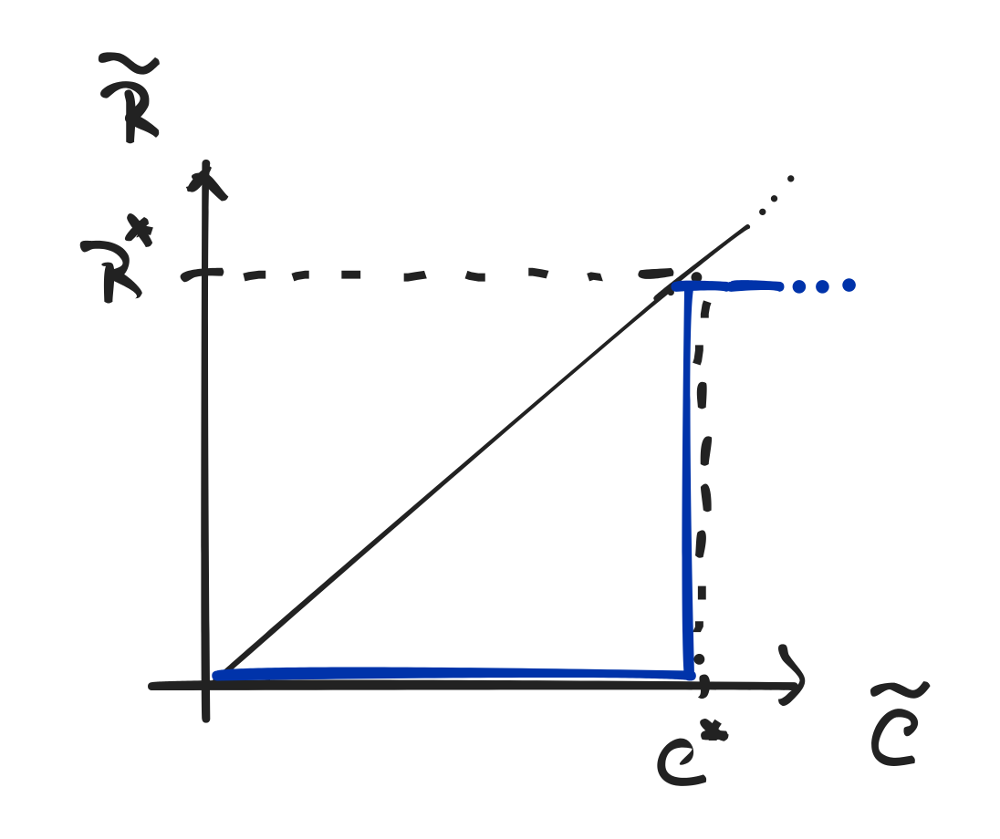
\includegraphics[scale=0.14]{pics/fg-sc.png}
		\caption{Cost/Reward in a FG protocol}
	\end{figure}
	\onslide<3->
	\column{0.5\textwidth}
		\begin{figure}
			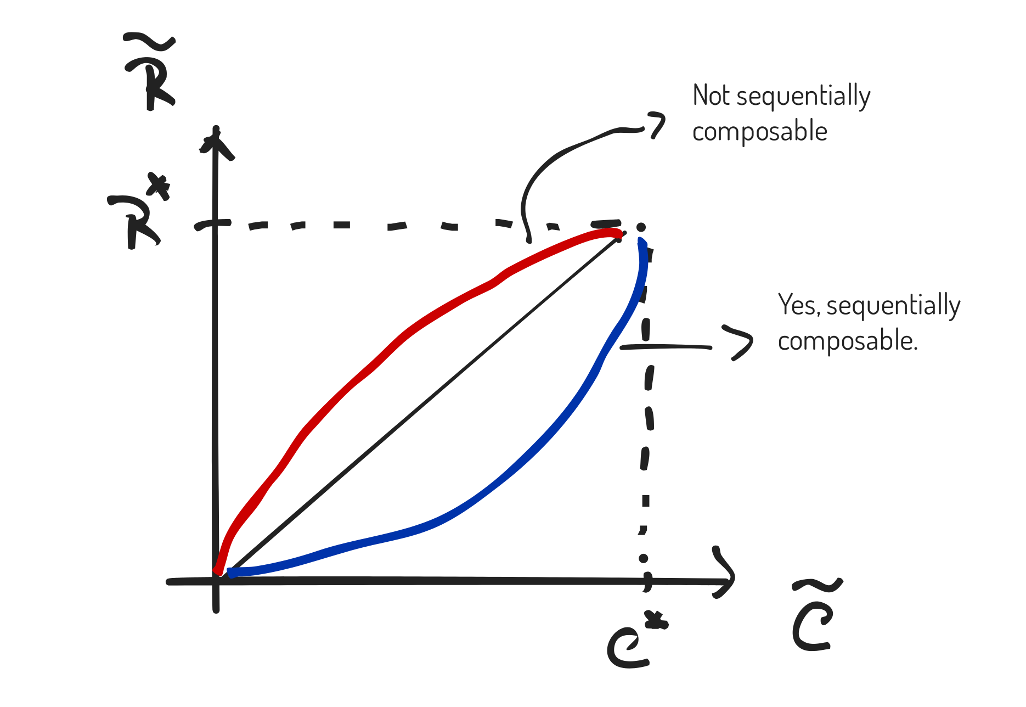
\includegraphics[scale=0.15]{pics/sc-char.png}
			\caption{Sequentially Composability (characterization)}
		\end{figure}
			
\end{columns}
\end{frame}

% == Our main result: FG VC against NC1 adversaries from minimal assumptions ==
\begin{frame}{Our FG Verifiable Computation Scheme}

\begin{block}{Our Main Result}
	A Non-Interactive Verifiable Computation Scheme secure against $\NC^1$ under $\L \not = \NC^1$.
\end{block}
\pause
\textbf{Properties:}
\begin{itemize}[<+- | alert@+>]
	\item I/O private;
	\item In the preprocessing model;
	\item Supports delegation of (a subset of) $\ACzt$.
\end{itemize}
\end{frame}


% == How to obtain this VC: HE + transformation ==
% Say here that another result will be for HE
\begin{frame}{How We Obtain Fine-Grained VC}
	Core of our approach is \cite{ckv10}:
	\begin{itemize}
		\item  Obtains VC from Homomorphic Encryption (HE)
	\end{itemize}
\end{frame}

\def\E{\func{E}}

% == Homomorphic Encryption ==
\begin{frame}{Homomorphic Encryption (HE)}
	\begin{center} \textbf{HE = PKE + Evaluation Function} \end{center}
	\begin{enumerate}
		\item $\func{KeyGen} \to (\pk, \sk)$
		\item $\func{Enc}_{\pk}(x) \to \E(x)$
		\item $\func{Dec}_{\sk}(\E(x)) \to x$
		\pause  
		\item $\func{Eval}_{\pk}(f, \E(x)) \to \E(f(x))$
	\end{enumerate}
	\pause
	\bigskip
	\begin{block}{Our Additional Result}
		HE against secure against $\NC^1$ adversaries under $\L \not = \NC^1$ supporting evaluation of (a subset of) $\ACzt$.
	\end{block}
\end{frame}

% == VC from HE ==
\begin{frame}[t]{VC from HE (\cite{ckv10})}
%	\begin{framed}
%	Core of our approach is \cite{ckv10}:
%	\begin{itemize}
%		\item  Obtains VC from Homomorphic Encryption (HE)
%	\end{itemize}
%	\end{framed}
%	\pause
\begin{columns}
		\column{0.65\textwidth}
	\procedure{Protocol from \cite{ckv10}}{%
		\textbf{Delegator} \> \> \textbf{Worker}  \\
		r \sample \bin^n\\
		y^*_0 \gets f(r)\\
		\vect{c}_0 \gets \E(r) \pclb
		\pcintertext[dotted]{End Offline Stage}
		\vect{c}_1 \gets \E(x)\\
		b \sample \bin \> \> \\
		\> \xrightarrow{\vect{c}_b, \vect{c}_{1-b}} \>  \\
		\> \> \vect{y}_0 \gets \func{Eval}(f, \vect{c}_0)    \\
		\> \> \vect{y}_1 \gets \func{Eval}(f, \vect{c}_1)    \\
		\> \xleftarrow{\vect{y}_b,\vect{y}_{1-b}} \>   \\
		\text{accept } \func{Dec}(\vect{y}_1) \text{ if } \func{Dec}(\vect{y}_0) = y^*_0 \> \>}
	\onslide<2->
	\column{0.35\textwidth}
	\textbf{Then:}
	\pause
	\begin{itemize}
		% TODO: Improve graphics so that changes are clear
		\item \textbf{To amplify error:} use random permutation\pause
		\item \textbf{To make reusable:} use HE  on top of construction.
	\end{itemize}
	
	\end{columns}
	% Scaling this up: error amplification (permutation); reusability
\end{frame}


% == VC from HE in low depth ==
\begin{frame}{Ensuring \cite{ckv10} works in low-depth}
	\textbf{Recall:} all our algorithms should run in $\NC^1$ and our verifier should be efficient.\pause
	
	\textbf{Some of the issues to take care of: }
	\begin{itemize}[<+- | alert@+>]
		\item How can we sample a random permutation in sufficiently low-depth?
		\item When using ``double'' HE, does double evaluation stay in $\NC^1$?
%		\item How to make sure it works when HE has \textit{randomized} decryption? (our decryption is randomized, but the original construction only works for deterministic)
		\item In the proof, does the security reduction stay in $\NC^1$?
	\end{itemize}
\end{frame}

% == HE against NC1 circuits==
\begin{frame}[t]{Obtaining Our HE scheme}
\begin{block}{Our Additional Result}
	HE against secure against $\NC^1$ adversaries under $\L \not = \NC^1$ supporting evaluation of (a subset of) $\ACzt$.
\end{block}
\pause
\bigskip
	\textbf{Our approach:}
	\begin{enumerate}[<+- | alert@+>]
		\item We start from the PKE secure against $\NC^1$ in \cite{fgcrypto};
		\item We apply relinearization techniques from \cite{fhe-lwe} to obtain HE;
		\begin{itemize}
			\item Can homomorphically evaluate polynomials of constant degree; 
		\end{itemize}
		\item We extend the class of functions we can evaluate homomorphically through degree reduction techniques from \cite{razborov1987lower}.
	\end{enumerate}\pause
	\textbf{Next, we see 1 and 2.}
\end{frame}

% == Description of DVV16 ==
\begin{frame}{PKE scheme from \cite{fgcrypto}}
	[TODO: Make more intuitive]
	\begin{itemize}
		\item $\PKEKeygen_{\sk}(\unlambda):$
		\begin{enumerate}
			\item Sample $(\M, \k) \gets \KSample(\unlambda)$;\\
			 {\color{red}(Property: if $\r$ random, $\transp{\r}  \M$ ``looks'' random to $\NC^1$ circuit)}
			\item Output $(\pk = \M, \sk = \k)$.
		\end{enumerate}
		\pause
		\item $\PKEEnc_{\pk}(\mu):$
		\begin{enumerate}
			\item Sample $\r \leftarrow_{\$} \bit^{\lambda}$;
			\item Let $\transp{t} = (0 \ \dots 0 \ 1) \in \bit^{\lambda}$;
			\item Output $\transp{\c} = \transp{\r}  \M + \mu\transp{\t}$.
		\end{enumerate}
		\pause
		\item $\PKEDec_{\sk}(\c):$
		\begin{enumerate}
			\item Output $\inprod{\k}{\c}$
		\end{enumerate}
		
	\end{itemize}
\end{frame}

\def\c{\vect{c}}
\def\cp{\vect{c'}}
\def\fc{f_{\c}}
\def\fcp{f_{\cp}}
\def\x{\vect{x}}

% == Description of relinearization ==
\begin{frame}{Relinearization step}
[TODO: Make all more intuitive]

 $  \fc(\x) = \inprod{\c}{\vect{x}} = \Sum c[i] x[i]$ \quad\quad\quad
 $  \fcp(\x) = \inprod{\cp}{\vect{x}} = \Sum c'[i] x[i]$
  \pause\\
 \medskip
 Homomorphic addition:
$$ \fc(\x)+\fcp(\x) = \inprod{\c+\cp}{\vect{x}}  = f_{\c+\cp}(\x) $$ 
\medskip 
\pause
Homomorphic multiplication:
 \begin{align*}
 \fc\cdot\fcp(\x)  & =   (\Sum c[i] x[i]) \cdot (\Sum c'[i]x[i]) \\
        				 & =  \Sum h_{i,j} x[i]x[j]   \quad\quad \small{( h_{i,j} \text{ obtained opening parenthesis})}
\end{align*}
\pause
\textbf{Problem:} now ciphertext this requires $\lambda^2$ bits.\pause

\textbf{Solution:} Provide $\vect{\rho}_{i,j} = \E(s[i]s[j])$ under a new secret key $\vect{t}$ as part of the public key.\pause
 
$
  \Sum h_{i,j} \vect{\rho}_{i,j}\pause  % TODO: Do bm
=  \Sum_{i,j,k} h_{i,j} \rho_{i,j}[k] t[k] \pause = \Sum_k t[k](\sum_{i,j} h_{i,j} \rho_{i,j}[k])\pause = f_{\c\cdot\cp}(\vect{t})
$
 
\end{frame}

\begin{frame}{Leveled Homomorphic Evaluation}
	[Intuition on doing relinearization at every level]
\end{frame}